\documentclass[onlytextwidth, aspectratio=169]{beamer}
\documentclass[onlytextwidth, aspectratio=169]{beamer}
\usepackage[utf8]{inputenc}
\usepackage{microtype}
\usepackage{amsmath}
\usepackage{amssymb}
\usepackage[nomessages]{fp} %\FPeval{\var-name}{2*sin(pi/6)}
\usepackage{siunitx} %units in math. eg 20\milli\meter
\usepackage{yhmath} % for arcs, overparenth command
\usepackage{tikz} %graphics
\usetikzlibrary{quotes, angles, arrows, arrows.meta}
%\usepackage{graphicx} already loaded by beamer class
%consider setting \graphicspath{{images/}}
%\parskip ?? to avoid paragraph indent
\usepackage{multicol} %may not need this package, just columns environment
\usepackage{venndiagram}

\subtitle[BECA]{Bronx Early College Academy}
\author[Huson]{Christopher J. Huson PhD}

\setbeamertemplate{headline}{\vskip2mm 
  \, BECA / \insertshortauthor \, / \inserttitle
  \hfill 
  \insertsection
  }

%Tick mark commands
\newcommand\ticks{}
  \def\ticks{{Bar[scale=2]}-{Bar[scale=2]}}
\newcommand\paraticks{}
  \def\paraticks{{Straight Barb[reversed, scale=2]}-{Straight Barb[scale=2]}}

\title{Geometry Unit 11: Regents review}
\date{9 June 2023}

\begin{document}
\frame{\titlepage}
\section[Outline]{}
\frame{\tableofcontents}

\section{1.1 Symmetry and dilation situations \hfill 9 June \,}
\begin{frame}{Learning Target: I can dilate a triangle}
  {HSG.SRT.B.5 Use similarity criteria for triangles to solve problems \hfill \alert{11.1 Friday 9 June}}
    Do Now
    \begin{enumerate}
      \item $\sin 55 = \cos (x+5)$. Find $x$.
      \item Find the equation of a line through $(3,1)$ with slope $m=2$.
      \item Find the slope of a line perpendicular to $y=\frac{1}{2}x+3$.
    \end{enumerate} \vspace{1cm}
    Lesson: Regents similar triangles \\
    Upload problem set Regents Aug '17\\[0.5cm]
    Homework: Deltamath problem set
\end{frame}

\begin{frame}{A dilation centered at the origin with scale factor $k=2$}
  \begin{columns}
    \column{0.6\textwidth}
    $\triangle ABC \rightarrow \triangle A'B'C'$ and $\triangle ABC \sim \triangle A'B'C'$\\[0.2cm]
    $A(0,0) \rightarrow A'(0,0)$\\
    $B(2,1) \rightarrow B'(4,2)$\\
    $C(1,-1) \rightarrow C'(2,-2)$ \vspace{0.3cm}
      \begin{description}
        \item[Use the letters] Corresponding parts are in order
        \item[Mappings] Write down what happens to each part using arrow notation $\rightarrow$
        \item[Scale factor] Calculate $\displaystyle k = \frac{new}{old}$ or $new = k \times old$
      \end{description}
    \column{0.4\textwidth}
    \begin{flushright}
      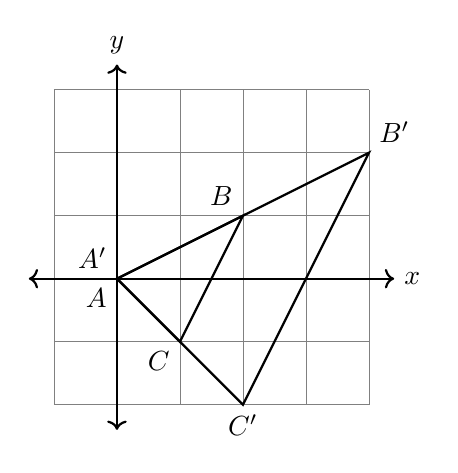
\begin{tikzpicture}[scale=0.8]
        \draw [help lines] (-1,-2) grid (4,3);
        \draw [thick, <->] (-1.4,0) -- (4.4,0) node [right] {$x$};
        \draw [thick, <->] (0,-2.4)--(0,3.4) node [above] {$y$};  
        \draw [thick]
          (0,0) node[below left] {$A$}--
          (2,1) node[above left] {$B$}--
          (1,-1) node[below left] {$C$}--cycle;
        \draw [thick]
          (0,0) node[above left] {$A'$}--
          (4,2) node[above right] {$B'$}--
          (2,-2) node[below] {$C'$}--cycle; 
      \end{tikzpicture}
    \end{flushright}
  \end{columns}
\end{frame}

\begin{frame}{``Solve'' a triangle by finding all of is sides' and angles' measures}
    Given $\triangle ABC \sim \triangle DEF$ \\[0.2cm]
    $BC=4$, $EF=6$, $AB=3$\\[0.2cm]
    m$\angle B = 55^\circ$, m$\angle D=70^\circ$\\[0.5cm]
    \begin{center}
      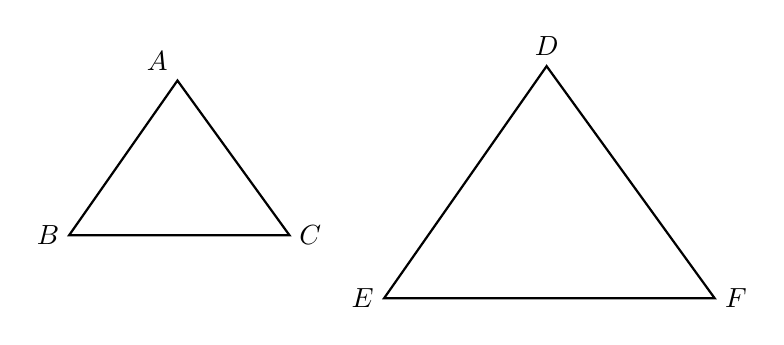
\begin{tikzpicture}[scale=0.8]
        \coordinate [label=above left:$A$](A) at (55:3);
        \coordinate [label=left:$B$](B) at (0, 0);
        \coordinate [label=right:$C$](C) at (0:3.5);
        \draw [thick] (A)--(B)--(C)--cycle;
        \draw [thick, xshift=5cm, yshift=-1cm, scale=1.5] 
          (55:3) node[above]{$D$}--
          (0,0) node[left]{$E$}--
          (0:3.5) node[right]{$F$}--cycle;
      \end{tikzpicture}
    \end{center}
\end{frame}

\begin{frame}{Rotation and dilation situations}
  {HSG.SRT.B.5 Use similarity criteria for triangles to solve problems \hfill \alert{9.7 Friday 24 March}}
  \begin{columns}
    \column{0.4\textwidth}
    What sequence of transformations map similar triangles $\triangle ABP \rightarrow \triangle JKP$? \\[0.5cm]
    Scale factor $k$, area scales by $k^2$, volume by $k^3$  \\[0.5cm]
    \column{0.6\textwidth}
    \begin{flushright}
      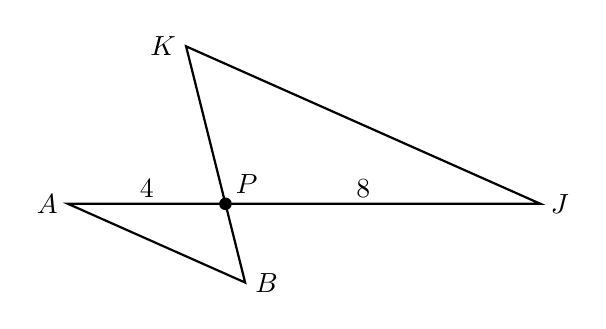
\begin{tikzpicture}[scale=1.0]
          \draw [thick]
            (0.25,-1)node[right]{$B$}--
            (-0.5,2)node[left]{$K$}--
            (4,0)node[right]{$J$}--
            (0,0)node[above right]{$P$}--
            (-2,0)node[left]{$A$}--cycle;
          \fill (0,0) circle (0.08);
          \node at (-1,0.2) {$4$};
          \node at (1.75,0.2) {$8$};
        \end{tikzpicture}
    \end{flushright}
  \end{columns}
\end{frame}

\begin{frame}{Triangle midline and medians create similar triangles}
  \begin{columns}
    \column{0.6\textwidth}
      \begin{description}
        \item[Midpoint] The point on a segment that divides the segment into two equal parts.
        \item[Midline] The line segment that connects the midpoints of two sides of a triangle.
        \onslide<2>{\item[Medians] Segments connecting a vertex to the midpoint of the opposite side.
        \item[Centroid] The point where the three medians intersect.}
      \end{description}
    \column{0.4\textwidth}
    \begin{flushright}
      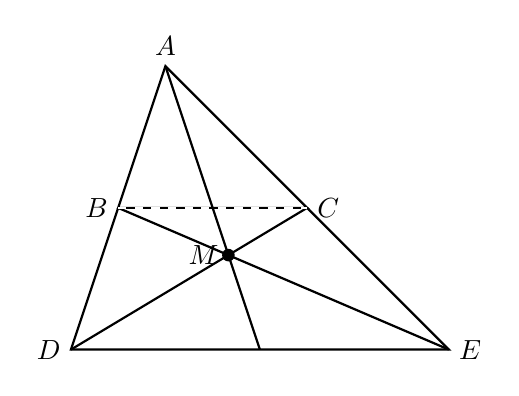
\begin{tikzpicture}[scale=0.4]
        \draw [thick]
        (0.5,1.5)node[left]{$B$}--
        (6.5,1.5)node[right]{$C$}--
        (2,6)node[above]{$A$}--cycle;
        \draw [thick] (0.5,1.5)--
          (-1,-3)node[left]{$D$}--
          (11,-3)node[right]{$E$}--(6.5,1.5);
        \pause
          \draw [thick] (2,6)--(5,-3);
          \draw [thick] (0.5,1.5)--(11,-3);
          \draw [thick] (6.5,1.5)--(-1,-3);
          \fill (4,0) circle (0.2)node[left]{$M$};
          \draw [dashed, thick, white] (0.5,1.5)--(6.5,1.5);
        %\node at (3,2.5)[below]{$7$};
        %\node at (2.1, 0)[above]{$4$};
        %\node at (-0.7, -1)[above]{$5$};
      \end{tikzpicture}
    \end{flushright}
  \end{columns}
\end{frame}

\begin{frame}{Overlapping triangles}
  \begin{columns}
    \column{0.4\textwidth}
    $\triangle ABC \cong \triangle ADE$ \\[0.5cm]
    $AB = 7$, $AC = 6$, $BD = 14$, $DE = 15$. \\[0.25cm]
    Find  $AD$ and the scale factor $k$. Then find $AE$ and $BC$. \vspace{1cm}
    \begin{enumerate}
      \item $AD=$
      \item $k=$
      \item $AE=$
      \item $BC=$ \vspace{1cm}
    \end{enumerate}
    \column{0.6\textwidth}
    \begin{flushright}
      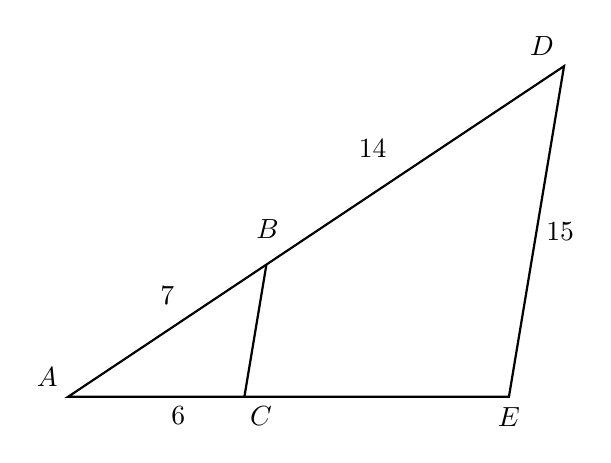
\begin{tikzpicture}[scale=0.7]
        \draw [-, thick] (0,0) node[above left]{$A$}--
        (8,0) node[below]{$E$}--
        (9,6) node[above left]{$D$}--cycle;
        \draw [thick] (3.2,0)--(3.6,2.4);
        \node at (3.5,0) [below]{$C$};
        \node at (4,2.7) [above left]{$B$};
        \node at (2, 0) [below]{$6$};
        \node at (1.8,1.5) [above]{$7$};
        \node at (8.5, 3) [right]{$15$};
        \node at (5.1, 4.5) [right]{$14$}; \vspace{1cm}
      \end{tikzpicture}
    \end{flushright}
  \end{columns}
\end{frame}

\begin{frame}{Overlapping, reflected triangles}
  $\triangle ABC$, with $\overline{AEB}$, $\overline{ADC}$. $AB=14$, $AD=8$, and $DE=4$.
  \begin{columns}
    \column{0.4\textwidth}
    $\angle ACB \cong \angle AED$ \vspace{0.25cm}
    \begin{enumerate}
      \item $\overline{AE} \rightarrow$ \rule{2cm}{0.15mm} \vspace{0.15cm}
      \item $\overline{AD} \rightarrow$ \rule{2cm}{0.15mm} \vspace{0.15cm}
      \item $\triangle ADE \sim$ \rule{2cm}{0.15mm} \vspace{0.15cm}
      \item What is the scale factor?\\[0.5cm] $k=$  \rule{2cm}{0.15mm}
      \item What is the length of $\overline{BC}$?  \vspace{1cm}
    \end{enumerate}
    \column{0.6\textwidth}
    \begin{flushright}
      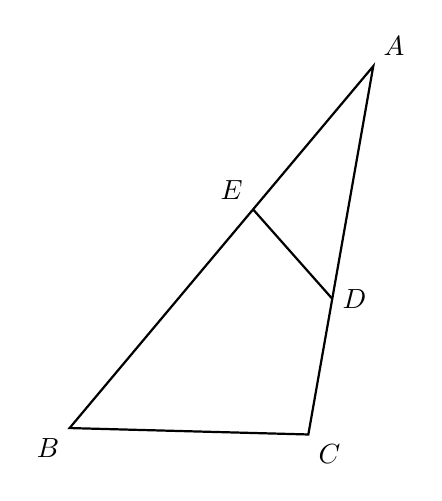
\begin{tikzpicture}[scale=1]
        \draw [thick]
        (0,0) node[above right] {$A$}--
        (230:6) node[below left] {$B$}--
        (260:4.75) node[below right] {$C$}--cycle;
        \draw [thick]
        (230:2.375) node[above left] {$E$}--
        (260:3) node[right] {$D$}--cycle;
      \end{tikzpicture}
    \end{flushright}
  \end{columns}
\end{frame}

\begin{frame}{Circle situations}
  \begin{columns}
    \column{0.4\textwidth}
    Chords $\overline{AE}$ and $\overline{BD}$ intersect at $C$ \\[0.5cm]
    $\triangle ABC \sim \triangle DEC$. \vspace{1cm}
    \begin{enumerate}
      \item Which angle is congruent to $\angle E$? 
      \item Given $BC=3$, and $EC=6$. Find the scale factor $k$.
      \item $AC=4$, find $CD$. \vspace{1cm}
    \end{enumerate}
    \column{0.6\textwidth}
    \begin{flushright}
      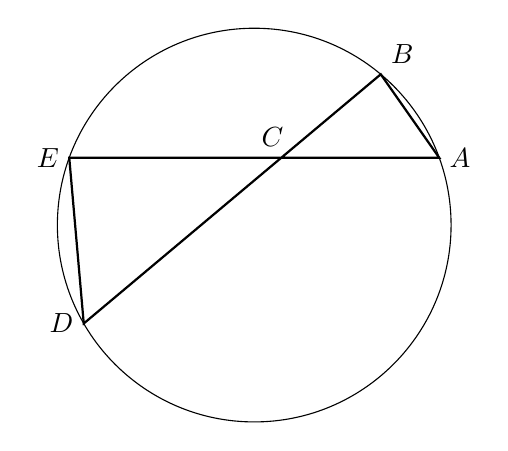
\begin{tikzpicture}[scale=.5]
        \draw (0,0) circle[radius=5];
        \draw [thick]
        (20:5) node[right] {$A$}--
        (160:5) node[left] {$E$}--
        (210:5) node[left] {$D$}--
        (50:5) node[above right] {$B$}--cycle;
        \draw (75:1.8) node[above] {$C$};
      \end{tikzpicture}
    \end{flushright}
  \end{columns}
\end{frame}

\begin{frame}{Proofs with similarity }
  \begin{columns}
    \column{0.6\textwidth}
      \begin{description}
        \item[Congruent angles] If two triangles have two corresponding angles congruent, then the triangles are similar. AA Similarity (abbreviated AA $\sim$)
        \item[Reflexive] Every angle is congruent to itself. The \emph{reflexive} property.
        \item[SSS $\sim$] Given $\triangle ABC$ with side lengths 5, 12, 13 and $\triangle ADE$ with 10, 24, 26.
        \item[``CPCTC''] Corresponding parts (sides or angles) of congruent triangles are congruent.
      \end{description}
    \column{0.4\textwidth}
    \begin{flushright}
      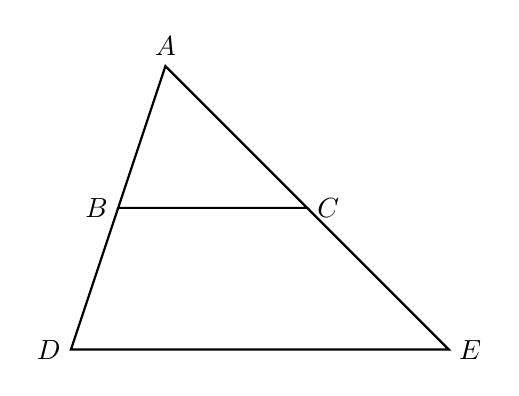
\begin{tikzpicture}[scale=0.4]
        \draw [thick]
        (0.5,1.5)node[left]{$B$}--
        (6.5,1.5)node[right]{$C$}--
        (2,6)node[above]{$A$}--cycle;
        \draw [thick] (0.5,1.5)--
          (-1,-3)node[left]{$D$}--
          (11,-3)node[right]{$E$}--(6.5,1.5);
      \end{tikzpicture}
    \end{flushright}
  \end{columns}
\end{frame}

\begin{frame}{Theorem of SSS Similarity and SAS Similarity}
  \begin{columns}
    \column{0.7\textwidth}
      \begin{description}
        \item[Proportion] Ratio or fraction. For a dilation, usually written as $k=\frac{\text{image}}{\text{preimage}}$.
        \item[SSS Similarity] If two triangles have two corresponding sides in the same proportion, then the triangles are similar.
        \item[SAS Similarity] If two triangles have two corresponding sides in the same proportion and their included angles are congruent, then the triangles are similar.
        \item[Included angle] The angle between two sides of a triangle.
      \end{description}
    \column{0.3\textwidth}
    \begin{flushright}
      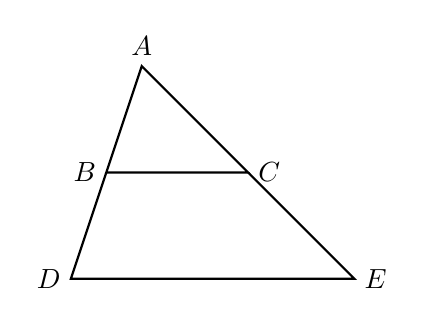
\begin{tikzpicture}[scale=0.3]
        \draw [thick]
        (0.5,1.5)node[left]{$B$}--
        (6.5,1.5)node[right]{$C$}--
        (2,6)node[above]{$A$}--cycle;
        \draw [thick] (0.5,1.5)--
          (-1,-3)node[left]{$D$}--
          (11,-3)node[right]{$E$}--(6.5,1.5);
      \end{tikzpicture}
    \end{flushright}
  \end{columns}
\end{frame}

\begin{frame}{Find the area of the large and small rectangles}
  {(use the areas of the small triangles)}
    \begin{flushright}
      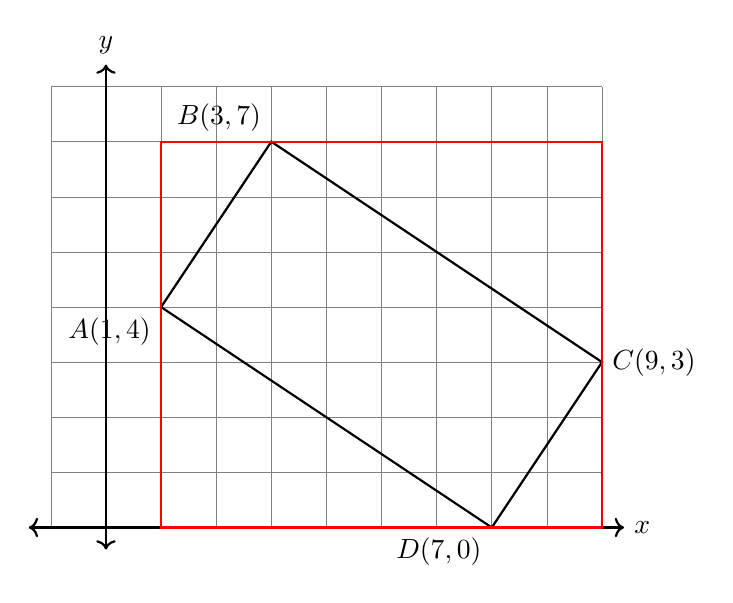
\begin{tikzpicture}[scale=0.7]
        \draw [help lines] (-1,0) grid (9,8);
        \draw [thick, <->] (-1.4,0) -- (9.4,0) node [right] {$x$};
        \draw [thick, <->] (0,-0.4)--(0,8.4) node [above] {$y$};  
        \draw [thick]
          (1,4) node[below left] {$A(1,4)$}--
          (3,7) node[above left] {$B(3,7)$}--
          (9,3) node[right] {$C(9,3)$}--
          (7,0) node[below left] {$D(7,0)$}--cycle;
        \draw [thick, red] (1,7)--(9,7)--(9,0)--(1,0)--cycle;
      \end{tikzpicture}
    \end{flushright}
\end{frame}

\end{document}
